\documentclass[11pt,a4paper]{article}

\usepackage[utf8]{inputenc}
\usepackage[T1]{fontenc}
\usepackage{geometry}
\usepackage{graphicx}
\usepackage{xcolor}
\usepackage{tikz}
\usepackage{hyperref}
\usepackage{fancyhdr}
\usepackage{titlesec}
\usepackage{helvet}
\usepackage{tabularx}
\usepackage{booktabs}
\renewcommand{\familydefault}{\sfdefault}

\usetikzlibrary{shapes.geometric, arrows.meta, positioning, fit, backgrounds}

\geometry{margin=0.75in}

% Sparrow Colors
\definecolor{sparrowPrimary}{HTML}{AA90FE}
\definecolor{sparrowDark}{HTML}{1B113A}
\definecolor{sparrowPurple}{HTML}{7c5ce8}
\definecolor{sparrowDeep}{HTML}{5b21b6}
\definecolor{elevenLabsBlue}{HTML}{0066FF}
\definecolor{googleRed}{HTML}{EA4335}
\definecolor{googleBlue}{HTML}{4285F4}
\definecolor{supabaseGreen}{HTML}{3ECF8E}
\definecolor{groqOrange}{HTML}{F55036}
\definecolor{vercelBlack}{HTML}{000000}

\hypersetup{colorlinks=true,linkcolor=sparrowPurple,urlcolor=sparrowPurple}

\pagestyle{fancy}
\fancyhf{}
\fancyhead[L]{\textcolor{sparrowDark}{\small Sparrow AI}}
\fancyhead[R]{\textcolor{sparrowDark}{\small System Architecture}}
\fancyfoot[C]{\textcolor{sparrowDark}{\thepage}}
\renewcommand{\headrulewidth}{0.5pt}
\renewcommand{\headrule}{\hbox to\headwidth{\color{sparrowPrimary}\leaders\hrule height \headrulewidth\hfill}}

\titleformat{\section}{\Large\bfseries\color{sparrowDark}}{\thesection}{1em}{}
\titleformat{\subsection}{\large\bfseries\color{sparrowPurple}}{\thesubsection}{1em}{}

\begin{document}

\begin{titlepage}
    \centering
    \vspace*{0.5cm}
    
\includegraphics[width=0.3\textwidth]{../public/Logo/sparrow-logo.png}
    \vspace{1cm}

    {\Huge\bfseries\textcolor{sparrowDark}{System Architecture}\par}
    \vspace{0.3cm}
    {\Large\textcolor{sparrowPurple}{Technical Infrastructure Overview}\par}
    \vspace{1.5cm}

    {\large\textcolor{sparrowDark}{AI Partner Catalyst Hackathon by Google Cloud}}
    \vfill
    {\small\textcolor{sparrowDark}{Version 1.0 | December 2025}}
\end{titlepage}

\section{Architecture Overview}

Sparrow AI is built on a modern, serverless architecture that leverages best-in-class AI services for real-time voice conversations, intelligent persona generation, and performance analysis.

\vspace{1em}

\begin{center}
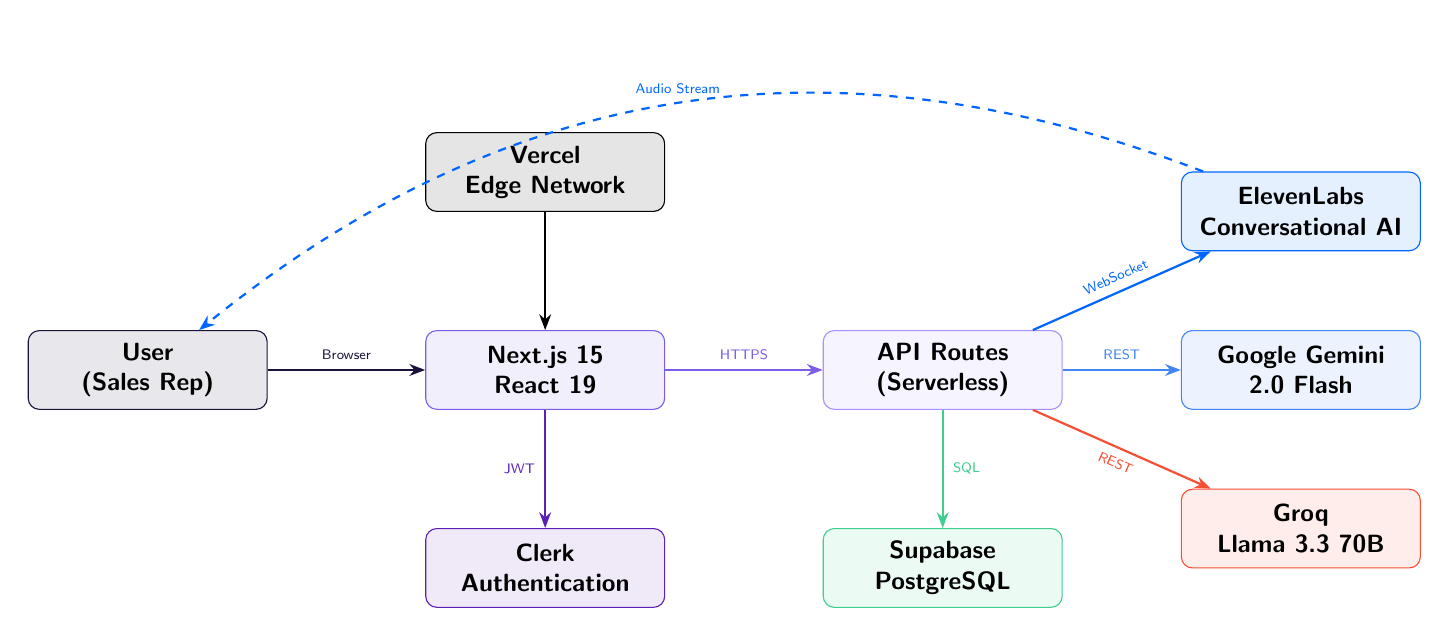
\begin{tikzpicture}[
    node distance=1.2cm and 1.5cm,
    box/.style={rectangle, rounded corners, draw=#1, fill=#1!10, text width=2.8cm, minimum height=1cm, align=center, font=\small\bfseries},
    arrow/.style={-{Stealth[length=2mm]}, thick, #1},
    label/.style={font=\tiny, align=center}
]

% User Layer
\node[box=sparrowDark] (user) {User\\(Sales Rep)};

% Frontend
\node[box=sparrowPurple, right=2cm of user] (frontend) {Next.js 15\\React 19};

% API Layer
\node[box=sparrowPrimary, right=2cm of frontend] (api) {API Routes\\(Serverless)};

% Voice AI - ElevenLabs (TOP - Prominent)
\node[box=elevenLabsBlue, above right=1cm and 1.5cm of api] (elevenlabs) {ElevenLabs\\Conversational AI};

% Google Cloud - Gemini
\node[box=googleBlue, right=1.5cm of api] (gemini) {Google Gemini\\2.0 Flash};

% Groq
\node[box=groqOrange, below right=1cm and 1.5cm of api] (groq) {Groq\\Llama 3.3 70B};

% Database
\node[box=supabaseGreen, below=1.5cm of api] (supabase) {Supabase\\PostgreSQL};

% Auth
\node[box=sparrowDeep, below=1.5cm of frontend] (clerk) {Clerk\\Authentication};

% Deployment
\node[box=vercelBlack, above=1.5cm of frontend] (vercel) {Vercel\\Edge Network};

% Arrows
\draw[arrow=sparrowDark] (user) -- node[above, label] {Browser} (frontend);
\draw[arrow=sparrowPurple] (frontend) -- node[above, label] {HTTPS} (api);
\draw[arrow=elevenLabsBlue] (api) -- node[above, label, sloped] {WebSocket} (elevenlabs);
\draw[arrow=googleBlue] (api) -- node[above, label] {REST} (gemini);
\draw[arrow=groqOrange] (api) -- node[below, label, sloped] {REST} (groq);
\draw[arrow=supabaseGreen] (api) -- node[right, label] {SQL} (supabase);
\draw[arrow=sparrowDeep] (frontend) -- node[left, label] {JWT} (clerk);
\draw[arrow=vercelBlack] (vercel) -- (frontend);

% WebSocket direct to user
\draw[arrow=elevenLabsBlue, dashed] (elevenlabs) to[bend right=30] node[above, label] {Audio Stream} (user);

\end{tikzpicture}
\end{center}

\section{Technology Stack}

\begin{tabularx}{\textwidth}{|l|l|X|}
\hline
\rowcolor{sparrowPrimary!20}
\textbf{Layer} & \textbf{Technology} & \textbf{Purpose} \\
\hline
Frontend & Next.js 15 + React 19 & Server components, App Router, real-time UI \\
\hline
Styling & Tailwind CSS 4 & Utility-first CSS, custom Sparrow theme \\
\hline
Voice AI & \textcolor{elevenLabsBlue}{\textbf{ElevenLabs}} & Real-time conversational AI with voice synthesis \\
\hline
AI/LLM & \textcolor{googleBlue}{\textbf{Google Gemini 2.0}} & Persona generation, deep analysis, feedback \\
\hline
Fast Inference & Groq (Llama 3.3 70B) & Real-time scoring during calls \\
\hline
Database & Supabase (PostgreSQL) & User data, call records, transcripts, analytics \\
\hline
Auth & Clerk & OAuth, user management, session handling \\
\hline
Hosting & Vercel & Edge deployment, serverless functions \\
\hline
\end{tabularx}

\section{Data Flow}

\subsection{Starting a Practice Call}

\begin{enumerate}
    \item User selects practice type (Cold Call / Discovery / Objection Gauntlet)
    \item \textbf{Gemini 2.0 Flash} generates a unique AI prospect persona
    \item Call record created in \textbf{Supabase}
    \item \textbf{ElevenLabs Conversational AI} session initialized with persona context
    \item WebSocket connection established for real-time audio
\end{enumerate}

\subsection{During the Call}

\begin{enumerate}
    \item User speaks $\rightarrow$ Audio streamed to \textbf{ElevenLabs}
    \item ElevenLabs STT $\rightarrow$ LLM processes with persona context $\rightarrow$ TTS response
    \item Audio response streamed back to user (sub-500ms latency)
    \item Transcript streamed to \textbf{Supabase Realtime} for live display
    \item \textbf{Groq} provides real-time coaching hints
\end{enumerate}

\subsection{Post-Call Analysis}

\begin{enumerate}
    \item Full transcript sent to \textbf{Gemini 2.0 Flash}
    \item Detailed scoring across 5 skill dimensions
    \item Timestamped feedback on key moments
    \item Results stored in \textbf{Supabase} for progress tracking
\end{enumerate}

\section{Integration Highlights}

\subsection{ElevenLabs Conversational AI (Primary Partner Integration)}

\begin{itemize}
    \item \textbf{Real-time voice conversations} with AI prospects
    \item \textbf{Dynamic voice selection} based on persona gender/personality
    \item \textbf{Custom system prompts} injected per conversation
    \item \textbf{Sub-500ms latency} for natural conversation flow
    \item \textbf{Multi-account failover} for high availability
\end{itemize}

\subsection{Google Cloud / Gemini (Required Integration)}

\begin{itemize}
    \item \textbf{Gemini 2.0 Flash} for intelligent persona generation
    \item \textbf{Deep conversation analysis} with structured JSON output
    \item \textbf{Skill-based scoring} with actionable feedback
    \item \textbf{Coach Sparrow} AI assistant powered by Gemini
\end{itemize}

\section{Scalability}

\begin{tabularx}{\textwidth}{|l|X|}
\hline
\rowcolor{sparrowPrimary!20}
\textbf{Component} & \textbf{Scaling Strategy} \\
\hline
Frontend & Vercel Edge Network - automatic global CDN \\
\hline
API & Serverless functions - scale to zero, infinite scale up \\
\hline
Voice AI & ElevenLabs managed infrastructure - enterprise SLA \\
\hline
Database & Supabase - managed PostgreSQL with connection pooling \\
\hline
AI/LLM & Google Cloud + Groq - managed, auto-scaling inference \\
\hline
\end{tabularx}

\vspace{2em}
\begin{center}
\textcolor{sparrowPurple}{\rule{0.5\textwidth}{0.5pt}}\\[1em]
\textcolor{sparrowDark}{\textit{Built for the AI Partner Catalyst Hackathon}}\\[0.5em]
\textcolor{sparrowPurple}{\textbf{Sparrow AI -- Never wing a call again.}}
\end{center}

\end{document}
